\section{Evaluation}
\label{sec:evaluation}


We evaluate \tool by implementing a word count program with prior text parsing, TPCH query 12 and a k-means application that uses array processing extension for \tool. \\

All experiments were performed on the Amazon EC2 Cloud, using 20 "m1.large" nodes as slaves and one as master. They each have 7.5 Gb of memory, 2 virtual cores with 2 EC2 compute units each, have \todo{xxx Gb} of instance storage and provide high throughput. Prior to the experiments we have measured up to 50 MB/s between two nodes. For the Hadoop experiments we used current Clouderas Hadoop distribution. We used Crunch version 0.2.4 and Scoobi 0.4.0. For Spark we used the Mesos \todo{cite} EC2 script to start a cluster, and then used Spark version 048276799 for our tests. We did not tweak Hadoop configuration beyond the default settings. For Spark we changed the default parallelism level to the number of machines in the cluster and increased the available memory to 6GB. 

\todo{Maybe move regex to optimizations}
% Regular expressions 

% Data Serialization
For serialization of data we used LMS code generation to achieve minimal overhead for both Crunch and Scoobi frameworks. We used generated versions since they outperformed the Kryo framework by a thin margin. For Spark we used Kryo. All benchmarks were run three times and in figures we present only the average. We also measured standard deviation but it is not displayed since it is smaller than 3\% of the job time in all experiments.

\begin{figure}[!hbt]
    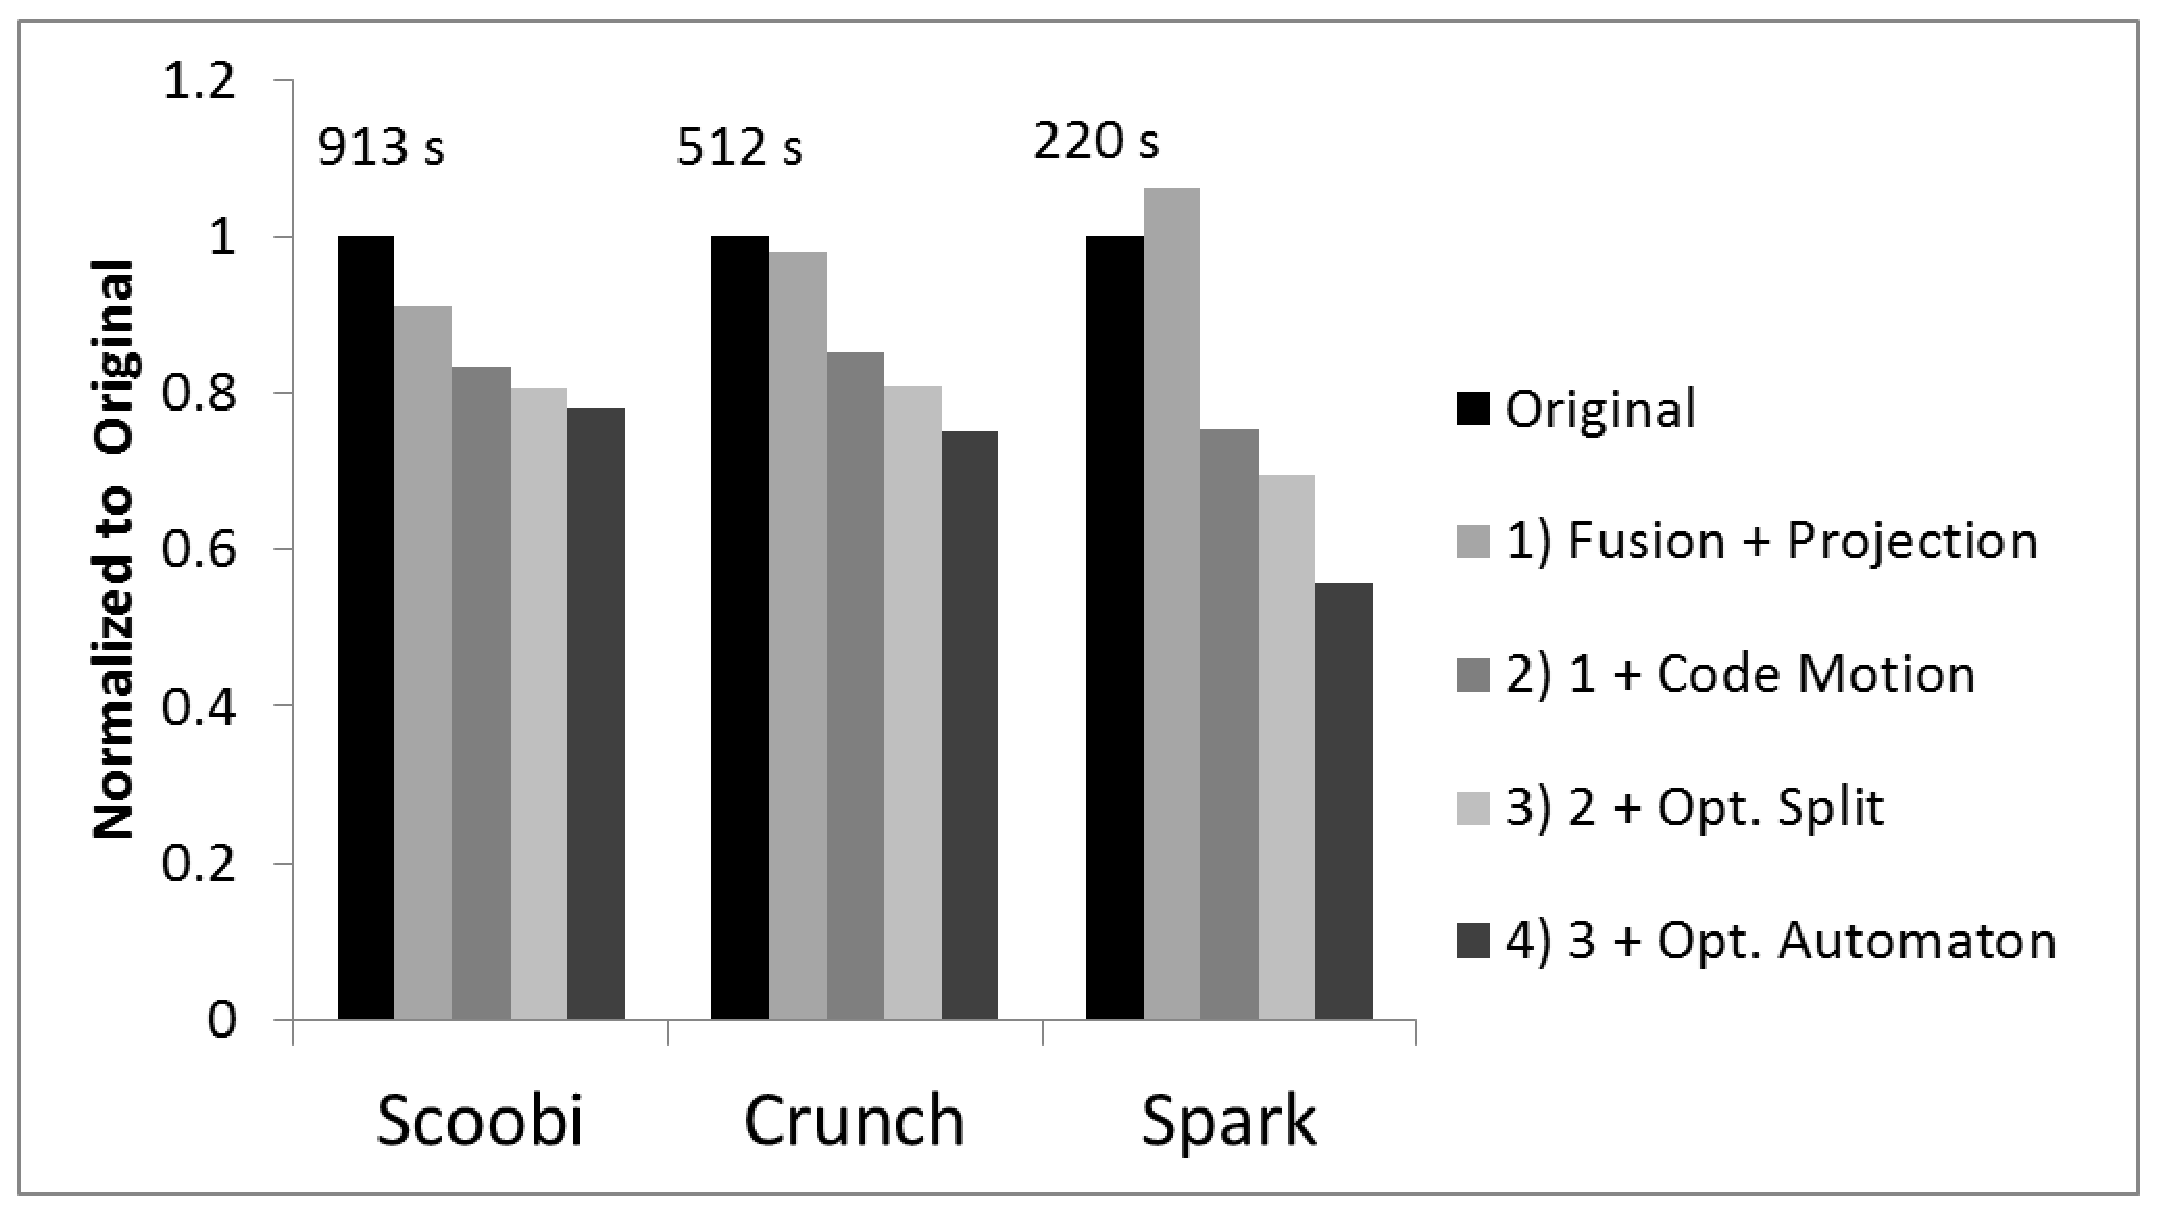
\includegraphics[width=8.6cm]{figures/word-count}
    \label{fig:word-count}\\%\vspace{10pt}
   \caption{KMeans}
\end{figure}

\begin{figure}[!hbt]
    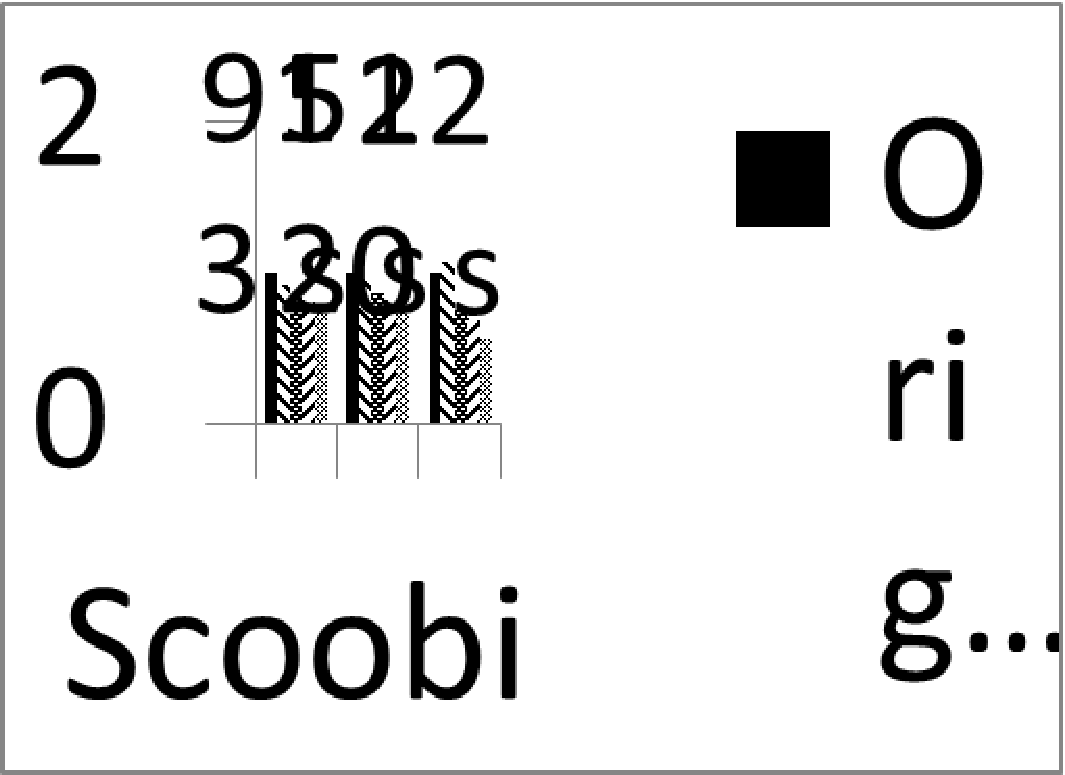
\includegraphics[width=8.6cm]{figures/k-means}
    \label{fig:k-means}\\%\vspace{10pt}
   \caption{KMeans}
\end{figure}

\begin{figure}[!hbt]
    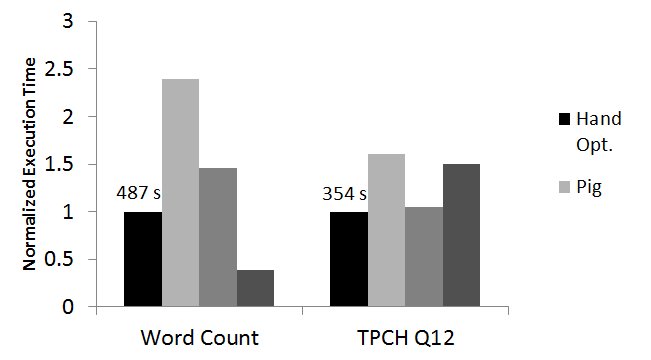
\includegraphics[width=8.6cm]{figures/pig}
    \label{fig:pig}\\%\vspace{10pt}
   \caption{KMeans}
\end{figure}

\begin{figure}[!hbt]
    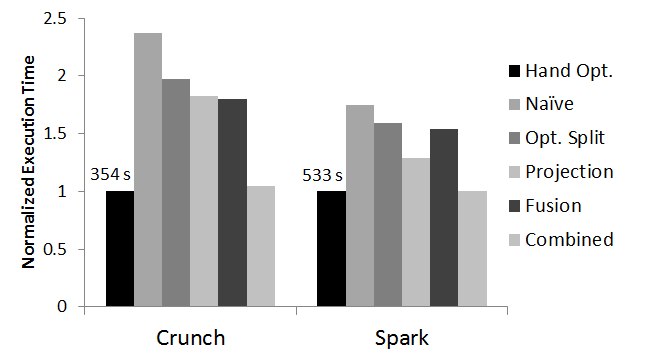
\includegraphics[width=8.6cm]{figures/tpch}
    \label{fig:tpch}\\%\vspace{10pt}
   \caption{KMeans}
\end{figure}

% WordCount
\subsection{Parsing and Word Count}
\label{subsec:parsing-word-count}
\todo{Stivo explain the regular expressions and what do we want to prove}

\todo{Stivo}
The word count is very heavy on the mapper side and only requires one shuffle stage. As input we use TODO, 62 Gb of tab separated values. It can not benefit from field reduction, but still uses the generated parsing method. We use multiple regex and evaluate different steps of the optimization for these regexes.

In figure \todo{\ref{}} show job times for different optimizations normalized to the unoptimized program version. In this benchmark we notice that code motion removes regular expressions automaton compilation from the hot loop. Performance improvements are so improvements are from \todo{75-82} in Scoobi, \todo{Crunch} and in Spark. Also, we notice significant fusion increase in Scoobi which indicates that the framework imposes additional overhead for declarative operations. 

In Spark, we notice larger benefits from optimizations. We believe that it has significantly smaller IO overhead so optimizations have more significant effect. For spark \tool performs . Also, we notice that fusion optimization is slower than the original program. This result does not match our experiments in a smaller cluster setup. We believe that it could be caused by a straggler node in the cloud environment.

% TPCH q12
\subsection{TPCH Query 12}
\label{subsec:tpch-query-12}

To evaluate effects of projection insertion we have run the TPCH query 12 which includes an expensive \code{join} operation and produces aggregates the whole result to just two values. As the data set we use 100 GB input data set generated by \todo{dbgen cite}. 

In figure \todo{\ref{}} we show job times for different optimizations normalized to the unoptimized program version. We notice that projection insertion gives \todo{from bla to bla} percent improvement performance on Crunch and \todo{from bla to bla} for Scoobi. In the figure we also show that projection insertion gives significantly better improvements in Spark than in Hadoop based frameworks. We believe that either network shuffle or the join operation are less optimal in Spark. \todo{Combined optimizations provide better improvements than a sum of individual ones. We explain that by the compiler optimizations shown in \todo{\ref{}}}


\subsection{Comparison with Pig}
\label{subsec:pig}
% Pig Comparison
In figure \todo{\ref{}} we compare most optimal versions of benchmarks to equivalent Pig programs. The figure is normalized to the Pig execution time and overall job time is stated above the bar. We notice that for TPCH query 12, combination of fusion, code motion and field reduction outperform Pig when the Crunch framework is used. For Crunch, field reduction alone is not enough to outperform the Pig framework. We believe that this result is caused by more efficient join operation in Pig. In future work we will investigate the cause for this. In the Word Count Crunch outperforms Pig even without any optimizations applied. With all optimizations the difference is significant. We explain this by the more optimal regular expressions processing support included in \tool. In regular expressions used in the benchmark Pig falls back to default Java regular expressions while \tool uses optimized automaton library. Scoobi framework performs slower than Pig in both benchmarks even with all optimizations applied.

For the sake of showing comparison between the Hadoop based frameworks and the Spark framework we include the Spark results in the graph. We see that in all cases except for unoptimized TPCH query 12 it significantly outperforms Hadoop based frameworks.

\subsection{Comparison with Pig}
\label{subsec:pig}

\subsection{K-Means}
\label{subsec:kmeans}
\todo{Stivo KMeans graph explanation}
% KMeans
We took a version of Sparks Kmeans application and ported it to our own language. This application can neither use field reduction nor can it really profit from loop fusion. We extended our DSL for this program with a highly optimized Vector class, which is compiled into an Array. As this program uses operations only available in spark, and it has been shown that spark outperforms hadoop by a large margin for it, we have only benchmarked it against the original spark implementation. As input we use synthetic data with 10 to 1000 dimensions, 100 centers and keeping the dimensions * points factor constant at TODO. \\
